\documentclass{article}
\usepackage{graphicx}
\usepackage{caption}
\usepackage{subcaption}
\begin{document}
	\section{first}
	Summary: Image Processing technology finds widespread use in various fields like Machine Learning, AI and computer vision. Images will be the next data. And developing projects on them is a great way to understand the concepts from the core. Building projects can be very challenging on image processing, but it is not very difficult due to the recent technological advancements and resources available.
	
	Here are some of the latest image processing projects you can build:
	
	Summary: Image Processing technology finds widespread use in various fields like Machine Learning, AI and computer vision. Images will be the next data. And developing projects on them is a great way to understand the concepts from the core. Building projects can be very challenging on image processing, but it is not very difficult due to the recent technological advancements and resources available.
	
	Here are some of the latest image processing projects you can build:
	Summary: Image Processing technology finds widespread use in various fields like Machine Learning, AI and computer vision. Images will be the next data. And developing projects on them is a great way to understand the concepts from the core. Building projects can be very challenging on image processing, but it is not very difficult due to the recent technological advancements and resources available.
	
	Here are some of the latest image processing projects you can build:
	
	Summary: Image Processing technology finds widespread use in various fields like Machine Learning, AI and computer vision. Images will be the next data. And developing projects on them is a great way to understand the concepts from the core. Building projects can be very challenging on image processing, but it is not very difficult due to the recent technological advancements and resources available.
	
	Here are some of the latest image processing projects you can build:
	
	\clearpage
	
	\begin{figure}[!hbtp]
		\centering
		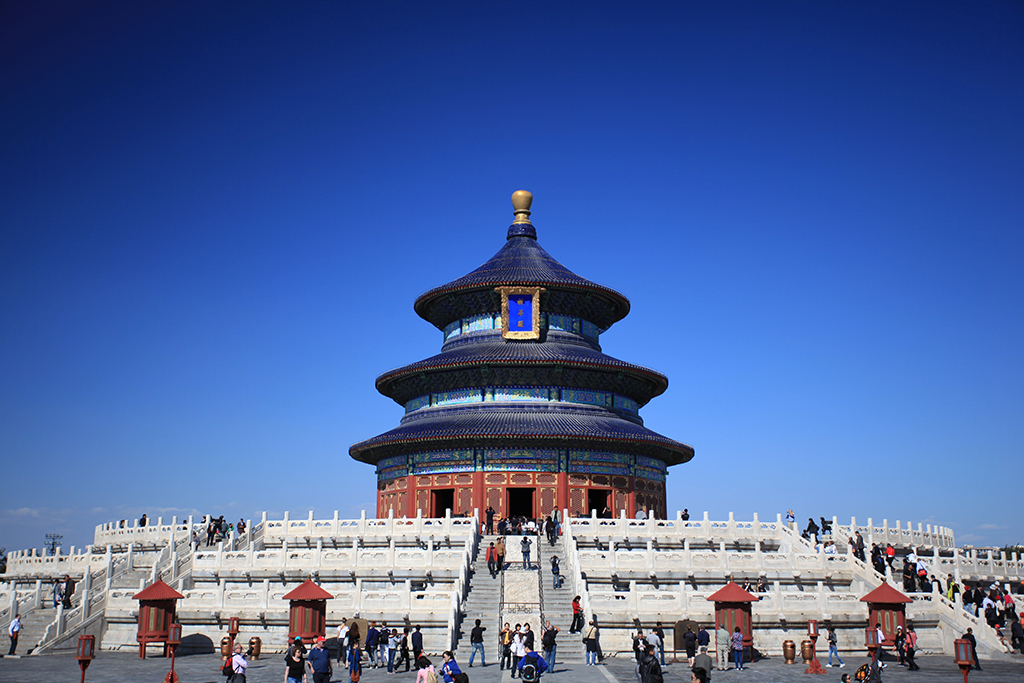
\includegraphics[width=\linewidth]{tiantan.jpg}
		\caption{tiantan}
		\label{fig:tiantan}
	\end{figure}
\clearpage
\begin{figure}[!hbtp]
	\centering
	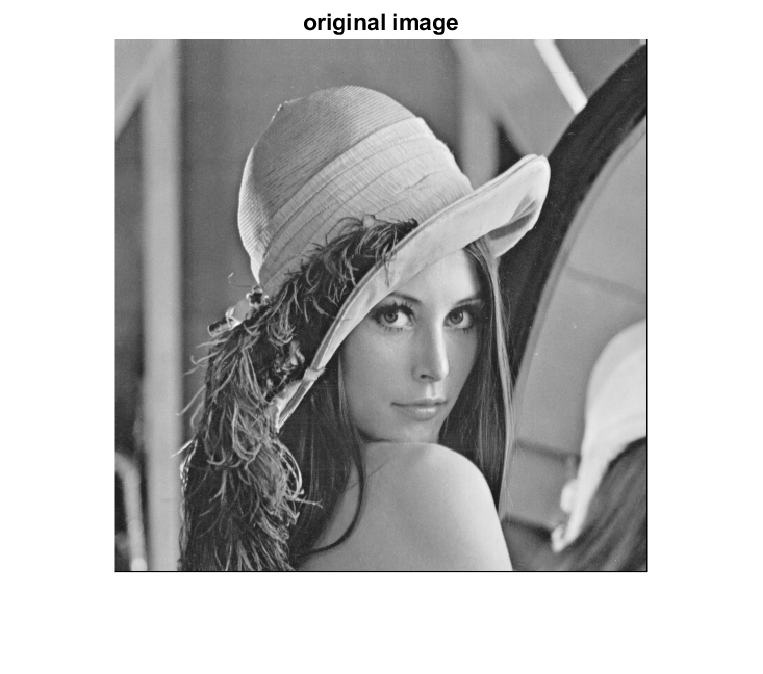
\includegraphics[width=\linewidth]{origin.png}
	\caption{tiantan}
	\label{fig:tiantan}
\end{figure}
\clearpage
\begin{figure}[!hbtp]
	\centering
	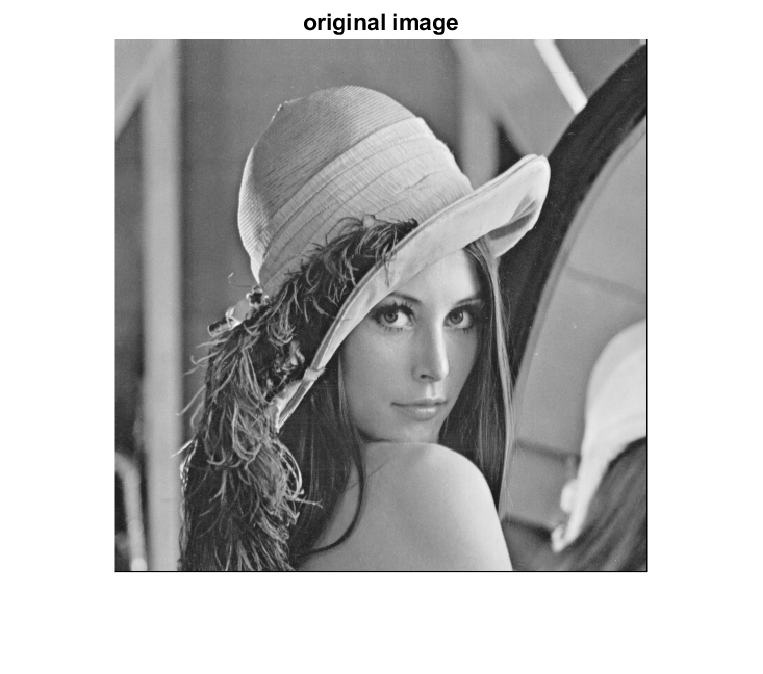
\includegraphics[width=\linewidth]{origin.png}
	\caption{tiantan}
	\label{fig:tiantan}
\end{figure}
\clearpage
\begin{figure}[!hbtp]
	\centering
	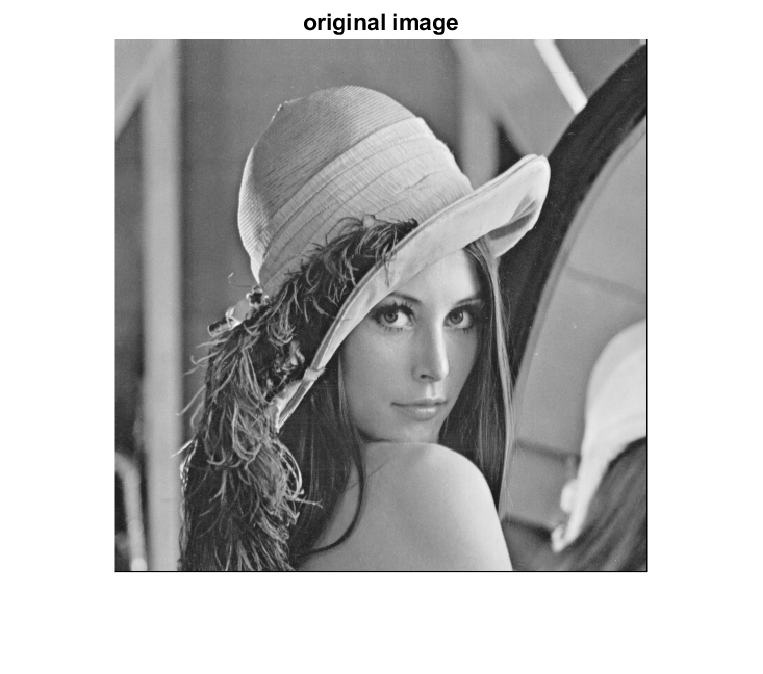
\includegraphics[height=0.5\linewidth]{origin.png}
	\caption{tiantan}
	\label{fig:tiantan}
\end{figure}
\section{second}
And developing projects on them is a great way to understand the concepts from the core. Building projects can be very challenging on image processing, but it is not very difficult due to the recent technological advancements and resources available.


\begin{figure}
	\centering
	\begin{subfigure}[!htbp]{0.5\textwidth}
		\centering
		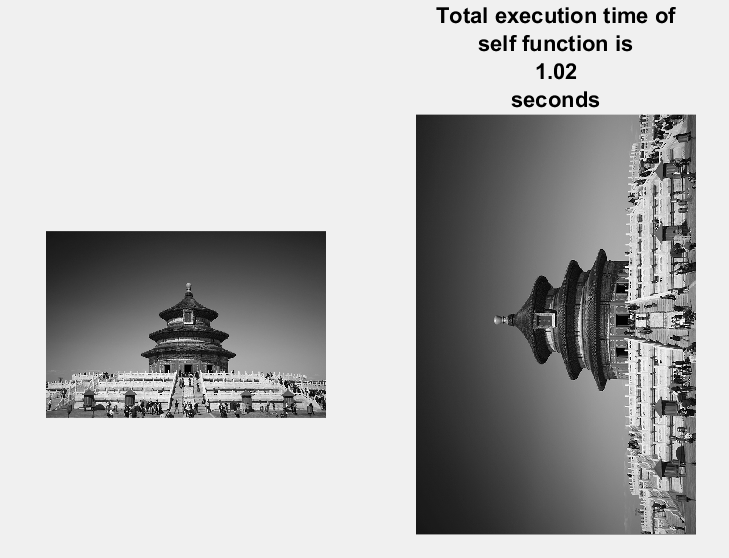
\includegraphics[width=0.8\textwidth]{selfRot.png}
		\caption{$y=x$}
		\label{fig:y equals x}
	\end{subfigure}
	\hfill
\begin{subfigure}[!htpb]{0.3\textwidth}
	\centering
	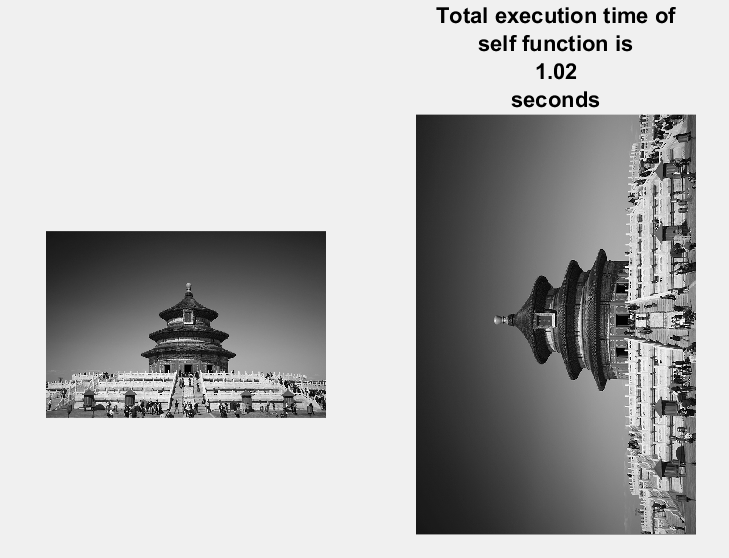
\includegraphics[width=\textwidth]{selfRot.png}
	\caption{$y=x$}
	\label{fig:y equals x}
\end{subfigure}
\caption{subfig}
\end{figure}
\clearpage
\begin{figure}[!bthp]
	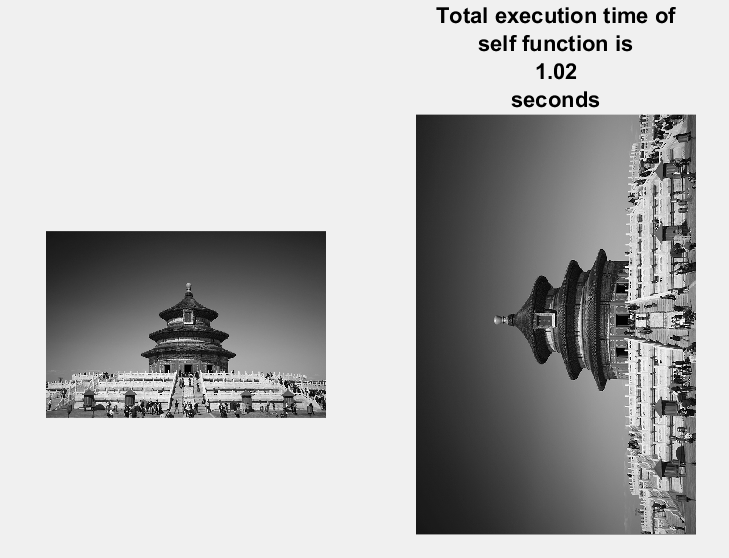
\includegraphics[width=\textwidth]{selfRot.png}
	\caption{lastfig}
\end{figure}
\section{three}
\end{document}
